%; whizzy chapter
% -initex iniptex -latex platex -format platex -bibtex jbibtex -fmt fmt
% 以上 whizzytex を使用する場合の設定。

%     Tokyo Debian Meeting resources
%     Copyright (C) 2012 Junichi Uekawa
%     Copyright (C) 2011 Nobuhiro Iwamatsu

%     This program is free software; you can redistribute it and/or modify
%     it under the terms of the GNU General Public License as published by
%     the Free Software Foundation; either version 2 of the License, or
%     (at your option) any later version.

%     This program is distributed in the hope that it will be useful,
%     but WITHOUT ANY WARRANTY; without even the implied warranty of
%     MERCHANTABILITY or FITNESS FOR A PARTICULAR PURPOSE.  See the
%     GNU General Public License for more details.

%     You should have received a copy of the GNU General Public License
%     along with this program; if not, write to the Free Software
%     Foundation, Inc., 51 Franklin St, Fifth Floor, Boston, MA  02110-1301 USA

%  preview (shell-command (concat "evince " (replace-regexp-in-string "tex$" "pdf"(buffer-file-name)) "&"))
% 画像ファイルを処理するためにはebbを利用してboundingboxを作成。
%(shell-command "cd image201205; ebb *.png")

%%ここからヘッダ開始。

\documentclass[mingoth,a4paper]{jsarticle}
\usepackage{monthlyreport}

% 日付を定義する、毎月変わります。
\newcommand{\debmtgyear}{2012}
\newcommand{\debmtgmonth}{5}
\newcommand{\debmtgdate}{19}
% (+ (* (- 2012 2005) 12) 5 -1) started from zero
\newcommand{\debmtgnumber}{88}

\begin{document}

\begin{titlepage}
\thispagestyle{empty}
% タイトルページ:編集必要な部分は最初のマクロに飛ばすこと

\vspace*{-2cm}
第\debmtgnumber{}回 東京エリア Debian 勉強会資料\\
\hspace*{-2cm}
\includegraphics[width=210mm]{image201003/debsen.eps}\\
\hfill{}\debmtgyear{}年\debmtgmonth{}月\debmtgdate{}日

% ここはアップデートすること
% 全角文字にしないとフォントのサイズが合わないので注意
% TODO(uekawa): なんでそうなるのか確認
\rotatebox{10}{\fontsize{32}{32} {\gt 特集: プログラミングの本を読んでみた}}

\vspace*{-2cm}
\hfill{}
\includegraphics[height=6cm]{image200502/openlogo-nd.eps}
\end{titlepage}

% Title should be in Japanese text so that we can use it as lint for PDF shiori.
\dancersection{はじめに}{上川 純一}

\begin{multicols}{2}
 

 今月のDebian勉強会へようこそ。これからDebianの世界にあしを踏み入れると
 いう方も、すでにどっぷりとつかっているという方も、月に一回Debianについ
 て語りませんか?

 Debian勉強会の目的は下記です。

 \begin{itemize}
 \item \underline{Debian Developer} (開発者)の育成。
 \item 日本語での「\underline{開発に関する情報}」を整理してまとめ、アップデートする。
 \item \underline{場}の提供。
 \begin{itemize}
  \item 普段ばらばらな場所にいる人々が face-to-face で出会える場を提供
	する。
  \item Debian のためになることを語る場を提供する。
  \item Debianについて語る場を提供する。
 \end{itemize}
 \end{itemize}		

 Debianの勉強会ということで究極的には参加者全員がDebian Packageをがりがり
 と作るスーパーハッカーになった姿を妄想しています。情報の共有・活用を通し
 て Debianの今後の能動的な展開への土台として、「場」としての空間を提供す
 るのが目的です。

\end{multicols}

\newpage

\begin{minipage}[b]{0.2\hsize}
 \definecolor{titleback}{gray}{0.9}
 \colorbox{titleback}{\rotatebox{90}{\fontsize{80}{80} {\gt デビアン勉強会} }}
\end{minipage}
\begin{minipage}[b]{0.8\hsize}
\hrule
\vspace{2mm}
\hrule
\begin{multicols}{2}
\tableofcontents
\end{multicols}
\vspace{2mm}
\hrule
\end{minipage}

\dancersection{事前課題}{上川 純一}

今回の事前課題は以下です:
\begin{enumerate}
 \item  Debian 勉強会参加者に紹介したい書籍を1冊以上挙げて、内容を簡単に紹介してください(特に技術書には限りません)。
 \item  あなたが何かスクリプト言語をプログラミング初心者にお勧めするとして「その言語を選んだ理由」と「最初の一歩として案内する書籍/サイト」を教えてください。
\end{enumerate}
この課題に対して提出いただいた内容は以下です。
\begin{multicols}{2}
{\small
 %; whizzy-master ../debianmeetingresume201205.tex
% $B0J>e$N@_Dj$r$7$F$$$k$?$a!"$3$N%U%!%$%k$G(B M-x whizzytex $B$9$k$H!"(Bwhizzytex$B$,MxMQ$G$-$^$9!#(B
%

\begin{prework}{ BeatenAvenue }

1.$B$*$9$9$aK\!'(B

$B!V(Bwindows$B%W%m%U%'%C%7%g%J%k%2!<%`%W%m%0%i%_%s%0(B($BA4#24,(B?)$B!W(B
DirectX$B4XO"$NFbMF$b$"$C$?5$$,$7$^$9$,(Bwin32API$B$K$D$$$F$NFbMF$,B?$+$C$?5$$,$7$^$9!#@N$NK\$G$9$,%?%9%/=hM}$N9M$(J}$J$I8=:_$G$bDLMQ$9$kItJ,$OB?$$$H;W$$$^$9!#$3$NK\$rGc$C$F$+$i(BC++$B$NJY6/$r;O$a$?$3$H$b$"$C$F!&!&!&8D?ME*$K;W$$=P$,$?$/$5$s$"$j$^$9!#(B

$B!V(BDirectX$B5U0z$-BgA4(B500$B$N6K0U!W(B
$BF~LgE*$JM%$7$$2r@b$+$i0lJbF'$_9~$s$@%W%i%9%"%k%U%!$^$GB7$C$F$$$^$9!#;DG0$J$,$i@dHG$G?^=q4[$+$i<Z$j$FFI$_$^$7$?!#(BDirectX9$B$N2r@b=q$G$O0lHV$h$$$b$N$+$H;W$$$^$9!#(B

$B!V(BGameProgrammingGems($B%7%j!<%:(B)$B!W(B
$B3$30$N%2!<%`%W%m%0%i%^$NJ}!9$,=q$$$?5-;v$r$^$H$a$?K\!#(B3$B4,$@$C$?$+$H;W$$(B
 $B$^$9$,(BNaughty Dog$B$NJ}$,=q$$$?(B"Jak and Daxter: The Precursor legacy"$B$G$N%^%C%W0\F0=hM}$K$D$$$F$NFbMF$,9%$-$G$9!#$*CMCJ0J>e!#(B

2.$B=i?4<T$K$*$9$9$a$9$k%9%/%j%W%H8@8l!'(B
Debian$B$H$OA4$/4X78$J$$$G$9$,(BDOS$B%P%C%A%U%!%$%k$H(BExcelVBA$B$N$A$g$C$H$7$?;H$$J}$O3P$($J$$$H;vL3;E;v$,?J$_$^$;$s!#2r@b%5%$%H$bB?$$$N$GIU$-$C$-$j$G65$($kI,MW$b$"$^$j$J$$$G$9!#(B
Linux$B$@$H(Bbash$B$N%9%/%j%W%H$J$s$G$7$g$&$+!#;d$,=i?4<T$J$N$G$=$l$7$+?($C$F$$$^$;$s!&!&!&!#(B
\end{prework}

\begin{prework}{ amotoki }

1. $B:rF|M'?M$+$i4+$a$i$l$F5$$K$J$C$F$$$k$N$,!V>pG.%W%i%0%i%^!<!W$G$9!#<+J,$N?M@8$r<+J,$G@Z$j3+$$$F$$$/$?$a$KI,MW$J$3$H$,J,$+$j$d$9$/@0M}$5$l$F$$$k$1$I!"<+J,$rA0$K?J$a$F$/$l$k>pG.$r46$8$?$H$N$3$H!#$5$C$=$/CmJ8$7$?!#(B

2. $B:#$*$9$9$a$9$k$H$7$?$i(BPython$B$r$*A&$a$7$^$9!#%*%V%8%'%/%H;X8~$b=q$-$d$9$$$7!"%i%$%V%i%j$b=<<B$7$F$$$F!"%^%K%e%"%k$b<BNc$,$=$m$C$F$$$k$N$G!"%W%m%0%i%_%s%0$r3X$s$G$$$/>e$G$h$$$H;W$$$^$9!#Bg$-$a$N(BOSS$B%W%m%8%'%/%H$G$b;H$o$l$F$$$k$N$G!"CN$C$F$*$$$FB;$9$k$3$H$b$"$j$^$;$s!#:G=i$N0lJb$H$7$F$O!V(BPython$B%A%e!<%H%j%"%k!W$,$h$$$H;W$$$^$9!#:#$G$b$H$-$I$-8+$k$3$H$,$"$j$^$9!#(B
\end{prework}

\begin{prework}{ $B5HLn(B(yy\_y\_ja\_jp) }

1. Git$B$K$h$k%P!<%8%g%s4IM}(B $B<B:]$N%W%m%8%'%/%H$G$N(BGit$B$NMxMQK!$,=q$+$l$F$$$k$h$&$G$9!%(B

2. $B%7%'%k%9%/%j%W%H(B
$B5$7Z$K;H$($k$+$i$G$9!%(B
bash(1), dash(1)
\end{prework}

\begin{prework}{ dictoss($B?yK\!!E5=<(B) }

1.$B!V%$%s%F%k(B $B%9%l%C%G%#%s%0!&%S%k%G%#%s%0!&%V%m%C%/(B -- $B%^%k%A%3%";~Be$N(BC++$BJBNs%W%m%0%i%_%s%0!W%*%i%$%j!<!&%8%c%Q%s!"(BJames Reinders$BCx(B
Intel$B$,3+H/$78=:_$O(BGPLv2$B$G8x3+$7$F$$$k(BC++$B$NJBNs7W;;MQ%i%$%V%i%j!V(BThreading Building Blocks$B!W$N2r@b$r9T$C$F$$$kK\!#%^%k%A%3%";~Be$NCf$GJ#?t$N(BCPU$B%3%"$r8zN(E*$K;HMQ$7$F7W;;@-G=$r>e$2$k$?$a$NCN<1$,5M$^$C$F$$$k!#$"$/$^$GC10l%N!<%I$G7W;;@-G=$r>e$2$k$?$a$N<jK!$G$"$j!"J#?t%N!<%I$G7W;;@-G=$r8~>e$5$;$k%/%i%9%?%j%s%05;=Q$NOC$G$O$J$$$N$GCm0U!#(B

2.$B$*4+$a$O(Bpython$B!#M}M3$O%W%m%0%i%_%s%0=i?4<T$H$$$&$3$H$G3+H/<T$K$h$C$F=q$-J}$K:90[$,=P$K$/$$J,(Bweb$B$G>R2p$5$l$F$$$k%3!<%I$KJJ$,$J$/$H$C$D$-$d$9$$$?$a!#(B
$B$*$9$9$a%5%$%H$O!"$&!<$s!"$J$s$G$7$g!)<+J,$OJL$N8@8l$,=q$1$k$h$&$K$J$C$F$+$i(Bpython$B$r;O$a$?$N$G(B"\url{http://www.python.jp/doc/release/}"$B$r3NG'$7$^$9!#(B
\end{prework}

\begin{prework}{ kamonshohei }

1. $B%7%'%k%9%/%j%W%H%7%'%k%9%/%j%W%H4pK\%j%U%!%l%s%9(B

2. $B%7%'%k%9%/%j%W%H$G$7$g$&$+!#%j%J%C%/%9$N%3%^%s%I$@$1$G!"$A$c$A$c$C$H<BAu$G$-$k<j7Z$5$,$$$$$G$9!#:G=i$N0lJb$G0FFb$9$k=q@R$O(B 1$B$G$"$2$?%7%'%k%9%/%j%W%H4pK\%l%U%!%l%s%9$G$9!#(B
\end{prework}

\begin{prework}{ emasaka }

1. $B%1%s!&%9%_%9!VC/$b65$($F$/$l$J$$@;=q$NFI$_J}!W!#@;=q$K=q$+$l$F$$$k$=$N$^$^$NJ8LL$r??LLL\$KFI$s$G%f!<%b%i%9$K>R2p!J!)!K$7$F$$$kK\!J(BDebian$B4X78$J$$!K(B

2. Bash$B$H=q$3$&$+$H;W$C$?$1$I(BRuby$B!#M}M3$O!V%*%V%8%'%/%H;X8~$r;H$C$F$b;H$o$J$/$F$b$$$$!W$G$O$J$/$F!V%*%V%8%'%/%H;X8~$r6/@)$5$l$k!W$+$i!#=q@R$O!V$?$N$7$$(BRuby$B!W(B

\end{prework}

\begin{prework}{ $BK\>1(B }

1. Debian $BJY6/2q;22C<T$K>R2p$7$?$$=q@R$r#1:}0J>e5s$2$F!"FbMF$r4JC1$K>R2p$7$F$/$@$5$$!#(B
$BDjHV$G$9$,!X%O%C%+!<$H2h2H!Y$H$+$I$&$G$7$g$&!#%*%?%/$N1eG0$,9~$a$i$l$F$$$^$9!#?F$H$7$F;R6!$N>-Mh$KIT0B$r46$8$^$9!#(B

2. $B$"$J$?$,2?$+%9%/%j%W%H8@8l$r%W%m%0%i%_%s%0=i?4<T$K$*4+$a$9$k$H$7$F!V$=$N8@8l$rA*$s$@M}M3!W$H!V:G=i$N0lJb$H$7$F0FFb$9$k=q@R!?%5%$%H!W$r65$($F$/$@$5$$!#(B
PHP$B$,$*$9$9$a$G$9!#$[$+$KHf$Y$F;E;v$,B?$=$&$H$$$&M}M3$G$9!#B?$$$+$I$&$+$O<B:]$N$H$3$m$o$+$j$^$;$s$,!"(B

\url{http://www.google.co.jp/trends/?q=PHP,+Perl,+Python,+Ruby,+Javascript,+Haskell&ctab=0&geo=jp&geor=all&date=ytd&sort=0}

$B$3$38+$k$HB?$=$&$G$9!#0FFb$9$k=q@R$H$7$FDjHV$O%^%s%b%9K\$@$H;W$$$^$9$,!"FI$s$@$3$H$O$"$j$^$;$s!#$=$7$F8E$$>pJs$+$b$7$l$^$;$s!#(B
$B0JA0!"$H$"$k(BPHP$BJ}LL$NJ}$H$*OC$7$9$k5!2q$,$"$j!"%*%i%$%j!<$NK\$O$A$g$C$H!DE*$J$3$H$rOC$7$?$i!"!V$"$"$$$&K\$b$$$$$+$J$H;W$C$F$^$9!W$H$$$o$l$^$7$?!#K]Lu<T$G$7$?!#(B

\end{prework}

\begin{prework}{ henrich }

1. $B!VF~Lg(BDebian$B%Q%C%1!<%8!W!#=qL>$+$iFbMF$,J,$+$k$+$H$O;W$$$^$9$,!"(BDebian$B%Q%C%1!<%8$N:n$jJ}$N=q@R$G$9!#B34)$,4|BT$5$l$^$9(B

2. Python $B$rA*$S$^$7$?!#(BPerl$B$O?M$K$h$C$F$H$F$b=q$-J}$,JQ$o$k$H$3$m$,$"$^$j4r$7$/$J$/!"(BRuby$B$O%P!<%8%g%s4V$N0\9T$,<c43MpK=$K46$8$i$l$?$N$G!#2?EY$b%W%m%0%i%_%s%0$K:C@^$7$F$$$k;d$G$9$,!":#2s(BPython$B$r3X$V$N$KA*$s$@!V=i$a$F$N%3%s%T%e!<%?%5%$%(%s%9!W$,$H$F$bNI$$=q@R$G$7$?!#(B
\end{prework}

\begin{prework}{ $BLnEg!!5.1Q(B }

1.$B!V%$%N%Y!<%7%g%s$N%8%l%s%^!W!J(BISBN10:4798100234)$B$H!"!V$N$&$@$^!W(B(ISBN10:4344015959)$B!#!V%$%N%Y!<%7%g%s$N%8%l%s%^!W$O!"5;=Q3W?7$,4{B8$N$b$N$r$V$A2u$7$F$$$/2aDx$K$*$$$F!"4{B85;=Q$K$*$$$FM%=($JAH?%$G$"$l$P$"$k$[$I5;=Q3W?7$K$D$$$F$$$1$J$/$J$C$F$7$^$&8=>]$rM}5M$a$G@bL@$7$?K\!#!V$N$&$@$^!W$O?M$N9TF0$K$*$$$F$O!"<B$O=,47$,@h$G$d$k5$$O8e$+$i$D$$$F$/$k$b$N$G$"$k$H$$$&;v$r@bL@$7$?K\!#(B

2. $B%W%m%0%i%_%s%0=i?4<T$K$O:#;~$N>u67$+$i(Bjavascript/HTML5$B$r4+$a$?$$$N$G$9$,!"4N?4$N<+J,$,L$I>2A!#:G=i$N0lJb$O%2!<%`M7$S$?$5$K%W%m%0%i%`3P$($?7P83$r85$K!"(B\url{http://wise9.jp/}$B!!$H!"!!(B\url{http://enchantjs.com/}$B!!$,$*$9$9$a$J$N$+$J!)(B
\end{prework}

\begin{prework}{ yamamoto }

1. Debian $BJY6/2q;22C<T$K>R2p$7$?$$=q@R$r#1:}0J>e5s$2$F!"FbMF$r4JC1$K>R2p$7$F$/$@$5$$!JFC$K5;=Q=q$K$O8B$j$^$;$s!K!#(B

$BM-L>$@$H;W$&$N$G!">R2p$9$k$[$I$N$3$H$O$J$$$+$b$7$l$^$;$s$,!"!VF~Lg(BUNIX$B%7%'%k%W%m%0%i%_%s%0(B-$B%7%'%k$N4pAC$+$i3X$V(BUNIX$B$N@$3&!!(BBruce Blinn $BCx!&;32<E/E5(B $BLu!W$r0&FI$7$F$$$^$9!#$^$"!"%7%'%k%9%/%j%W%H%W%m%0%i%_%s%0$r%7%'%k%W%m%0%i%_%s%0$H8@$C$F$$$k%?%$%H%k(B ($BL^O@%7%'%k<+BN$N2r@b$b$"$j$^$9$1$I$M(B) $B$O%"%l$G$9$,!"(BB$B%7%'%k$N%9%/%j%W%H$r=q$/$H$-$K$ONI$/3+$$$F$$$^$9!#(B

2. $B$"$J$?$,2?$+%9%/%j%W%H8@8l$r%W%m%0%i%_%s%0=i?4<T$K$*4+$a$9$k$H$7$F!V$=$N8@8l$rA*$s$@M}M3!W$H!V:G=i$N0lJb$H$7$F0FFb$9$k=q@R!?%5%$%H!W$r65$($F$/$@$5$$!#(B

\#!/bin/sh $BK|:P!*(B
$B$I$3$G$bBg35F0$/$+$i$*$9$9$a!#(B
B$B%7%'%k$N:nK!$K=>$C$F$$$l$P!":#$N(Bdash$B$J$iBgBNF0$/!)$_$?$$(B ($BL$3NG'(B)$B!#(B
$B$@$a$J$i!!(B\#!/bin/bash$B$G!#(B
$B$H$+$$$$$J$,$i$b!"$*$$$i$N%7%'%k%9%/%j%W%H$K$O30It%3%^%s%I%P%j%P%jF~$l$F$^$9$1$I!#(B($B$&$R(B

$B>e5-$N=q@R$G$b$$$$$G$9$,!"$0$0$k$5$s$K$*;G$$$7$?$i!";29M$K$J$k%5%$%H$O;3$[$I=P$F$/$k$G$7$g$&!#(B
\end{prework}

}
\end{multicols}

\dancersection{最近のDebian関連のミーティング報告}{上川 純一}
\subsection{東京エリアDebian勉強会87回目報告}

% (query-replace-regexp "<.*?>" "")
% (query-replace-regexp "^[	 ]\+" "")
2012年4月のDebian勉強会は新宿での開催でした。

Android tabletからDebianをネイティブブートさせるという話題。
debian-installer-6.0-netboot-armelにARMのインストーラーがはいっていて、
qemu-system-armの起動に活用できるようになっているというのに感動。起動イメー
ジの試行錯誤にQEMUを使えるというのが良いですね。

DebianでのNode.jsの最近の事情について上川が発表しました。先月はパッケージ
がちゃんとインストールできませんでしたが、今月はできるようになってますね。

\dancersection{Debian Trivia Quiz}{上川 純一}

ところで、みなさん Debian 関連の話題においついていますか?Debian関連の話
題はメーリングリストをよんでいると追跡できます。ただよんでいるだけではは
りあいがないので、理解度のテストをします。特に一人だけでは意味がわからな
いところもあるかも知れません。みんなで一緒に読んでみましょう。

今回の出題範囲は\url{debian-devel-announce@lists.debian.org} や \url{debian-devel@lists.debian.org}に投稿された
内容とDebian Project Newsからです。

\begin{multicols}{2}
 %; whizzy-master ../debianmeetingresume201205.tex
% 以上の設定をしているため、このファイルで M-x whizzytex すると、whizzytexが利用できます。
%

\santaku
{Debian installer 7.0 alpha 1 のリリース日は}
{5/13}
{6/13}
{4/13}
{A}
{Wheezyのインストーラーのアルファリリースが出たので皆さん試してください。}

\santaku
{Cyril Brulebが6月にWheezyをフリーズすると発表したが、Transitionの締め切りはいつだといっているか}
{5月13日}
{6月10日}
{5月20日}
{C}
{Transitionするなら5月20日までにバグをファイルしておけとのこと。Transitionというのはざっくりというと多数のパッケージが相互に依存しているような変更。例えば、ライブラリのABIが変わるだとか。}

\end{multicols}

%-------------------------------------------------------------------------------
\dancersection{Python初心者が「Pythonプロフェッショナルプログラミング」を読んでみた}{やまねひでき}
%-------------------------------------------------------------------------------
\label{sec:python-professional-programing}
\index{python}

わたくし、「Pythonプロフェッショナルプログラミング」という書籍を先日購入しました。私自身はまだ3月末ぐらいにPythonの入門から始めたばかりで本当はPythonビギナーズプログラミングが欲しいのですが、まだ世の中にはそのような本はありませんし、この書籍自体は評判が良かったので…

で、実際読んでみて中々実践的というか環境構築などで参考になることが多々ありました。しかし、もうちょっと突っ込んでみたいなぁ、というところがいくつかあったので、Debianパッケージ方面からの見方として取り上げてみようと思います。この書籍自体ではUbuntu11.10を使っていますが、私のDebian unstableのやり方でも大体のところはそのまま応用が効くはずです。


\subsection{なるべくディストリビューションのパッケージを使いたい}

PythonにはPythonパッケージがあり、配布サイトPyPIがあります。PerlにCPAN、Rubyにgems、RにCRANみたいなものですね。で、このPythonパッケージを導入するのにpipというツールを使う旨説明があるのですが(P.4)、githubからwgetして、インストールスクリプトをsudoで実行しています。\verb!/usr/local! 以下にツールが入るわけです。書籍全体でこのpipを使ったインストールを勧めていますが、これは美しくない。Debianパッケージにpython-pipがあるので、そちらを入れてもいいんじゃないかと思います\footnote{pipは若干バージョンが古いですが、そんなに不都合もないかなーと。古いのが嫌ならローカルにアップデートパッケージ作っちゃうのが吉。}。それからユーザーの HOME 以下にパッケージをインストールするvirtualenvというツールがあります。これもpython-virtualenvパッケージを入れて対応します。この後は、virtualenvでユーザーのPython環境にpipでパッケージを入れていってもいいかな、と思います。便利ツールとして紹介されているvirtualenvwrapperもvirtualenvwrapperパッケージがありますのでそれを入れちゃいましょう。

\begin{commandline}
$ sudo apt-get install python-pip python-virtualenv virtualenvwrapper
\end{commandline}

この後でユーザー個人のPython仮想環境下にpipでPythonパッケージをガシガシ入れていくのはありだと思います。


\subsection{複数バージョンのPythonを使う、のはいいけど。}

Python2.5をインストールするのに公式のパッケージリポジトリからだと11.10に入れられないよ、ということが書いてあります(P.11)。ここでPPAからインストールするか、ソースからインストールするかという選択になっています。業務で使う場合、そのPPAがどれほど信用できるかを説明するのが難しいように思います。自己責任で、って書いてありますが、大抵盲目的にそのPPA信用しちゃうような…。古いバージョンを使わなきゃダメ、という場合、私だったら「debootstrapで古い環境を作る」というやり方でやります(debootstrapについては後ほど述べます)。


それからソースからPython2.5を入れる説明ですが、

\begin{commandline}
$ wget http://www.python.org/ftp/python/2.5.6/Python-2.5.6.tgz
$ tar -xvzf Python-2.5.6.tgz
$ cd Python-2.5.6
$ LDFLAGS="-L/usr/lib/x86_64-linux-gnu" ./configure
$ make
$ sudo make install
(「Pythonプロフェッショナルプログラミング」より引用)
\end{commandline}

という説明になっています。i386だとパス変わるよね…というのは読み取れるのか若干心配な所です。プロフェッショナルだからいいのかな?必要な依存パッケージについては、最初の方のページで

\begin{commandline}
$ sudo aptitude -y install build-essential
$ sudo aptitude -y install libsqlite3-dev
$ sudo aptitude -y install libreadline6-dev
$ sudo aptitude -y install libgdbm-dev
$ sudo aptitude -y install zlib1g-dev
$ sudo aptitude -y install libbz2-dev
$ sudo aptitude -y install sqlite3
$ sudo aptitude -y install tk-dev
$ sudo aptitude -y install zip
(「Pythonプロフェッショナルプログラミング」より引用)
\end{commandline}
%$ -- for emacs

となっていました。あぁ、これはイケてない。パッケージビルド用のパッケージ取得は build-dep するべきです。Squeezeではまだ2.5のバイナリパッケージが手に入るので、ここでは2.4をターゲットに作業してみましょう。こんな風に\footnote{ここのパッケージ名指定は、本当はpython2.4にしたいけど無いので2.5にしています。多少の差は後で修正。}。

\begin{commandline}
$ sudo apt-get build-dep python2.5
\end{commandline}

これでPythonをビルドするときに必要な依存パッケージはすべてインストールされます。あ、apt lineにdeb-srcラインを追加を忘れずに。このやり方なら、Python以外のソフトウェアパッケージでもバージョンが変わっても大体応用が効きます。

そして「ソースからそのまま入れると\verb!/usr/local!以下に入るから、pythonとだけ打つとPATHの優先度でソースから入れたPython2.5が起動する」…という説明が…そんな罠作らない方がいいじゃないですかー。私ならソースから入れるのなら「Python2.5のDebianパッケージを利用環境用にリビルドしていれる」をやります。PTSのPython2.4のページ \footnote{\url{http://packages.qa.debian.org/p/python2.4.html}} からソースパッケージのdscファイルが取得できるので、これをdevscriptsパッケージのdgetコマンドで取得します。

\begin{commandline}
$ sudo apt-get install devscripts 
$ dget http://cdn.debian.net/debian//python2.4_2.4.6-1+lenny1.dsc
dget: retrieving http://cdn.debian.net/debian//python2.4_2.4.6-1+lenny1.dsc
--2012-05-04 03:59:21--  http://cdn.debian.net/debian//python2.4_2.4.6-1+lenny1.dsc
Resolving cdn.debian.net... 150.65.7.130
Connecting to cdn.debian.net|150.65.7.130|:80... connected.
HTTP request sent, awaiting response... 404 Not Found
2012-05-04 03:59:22 ERROR 404: Not Found.

dget: wget python2.4_2.4.6-1+lenny1.dsc http://cdn.debian.net/debian//python2.4_2.4.6-1+lenny1.dsc failed
\end{commandline}

あれ、oldstableだとリンクが切れちゃいますか\footnote{これはバグ報告しましょう}。しょうがないので、archive.debian.orgに切り替えてみます。
\begin{commandline}
$ dget http://archive.debian.org/debian/pool/main/p/python2.4/python2.4_2.4.6-1+lenny1.dsc
\end{commandline}
%$ -- for emacs

これでPython2.4のソースパッケージが取得できました。ビルド用の依存パッケージは既に入れているので、ソースパッケージのchangelogに一言書いてビルドすれば独自リビジョンをつけた deb パッケージが出来上がりますので、dpkgで入れちゃえば良いでしょう(後で述べますがaptを使ってインストールも可能です)。

\begin{commandline}
$ dpkg-source -x python2.4_2.4.6-1+lenny1.dsc
$ cd python2.4-2.4.6/
$ export DEBFULLNAME="Hideki Yamane"
$ export DEBEMAIL="henrich@debian.org"
$ dch --bpo "rebuild package for my own environment"
$ debuild -us -uc
dpkg-checkbuilddeps: Unmet build dependencies: libreadline5-dev tk8.4-dev libdb4.5-dev emacs22
dpkg-buildpackage: warning: Build dependencies/conflicts unsatisfied; aborting.
\end{commandline}

あれ、依存関係が満たせない。python2.5と比較してちゃちゃっと変更しましょうか。apt-get source python2.5 として、diff取ります。

\begin{commandline}
--- python2.4-2.4.6/debian/control	2012-05-04 04:09:00.000000000 +0000
+++ python2.5-2.5.5/debian/control	2012-05-04 04:13:06.000000000 +0000
@@ -1,82 +1,96 @@
-Source: python2.4
+Source: python2.5
 Section: python
 Priority: optional
 Maintainer: Matthias Klose <doko@debian.org>
-Build-Depends: debhelper (>= 5), autoconf, libreadline5-dev, libncursesw5-dev (>= 5.3), tk8.4-dev, libdb4.5-dev, zlib1g-dev, 
libgdbm-dev, blt-dev (>= 2.4z), libssl-dev, sharutils, libbz2-dev, libbluetooth-dev [!hurd-i386 !kfreebsd-i386 
!kfreebsd-amd64], locales, mime-support, libgpm2 [!hurd-i386 !kfreebsd-i386 !kfreebsd-amd64], netbase, lsb-release, bzip2
-Build-Depends-Indep: libhtml-tree-perl, texlive-latex-recommended, texinfo, emacs22, debiandoc-sgml
-Build-Conflicts: tcl8.3-dev, tk8.3-dev, python2.4-xml, python-xml
-XS-Python-Version: 2.4
-Standards-Version: 3.8.0
+Build-Depends: debhelper (>= 5), autoconf, libreadline-dev, libncursesw5-dev (>= 5.3), tk8.5-dev, libdb4.8-dev, zlib1g-dev, 
libgdbm-dev, blt-dev (>= 2.4z), libssl-dev, libbz2-dev, libbluetooth-dev [!hurd-i386 !kfreebsd-i386 !kfreebsd-amd64], 
locales [!avr32 !m68k], libsqlite3-dev, libffi-dev (>= 3.0.5-2), mime-support, libgpm2 [!hurd-i386 !kfreebsd-i386
 !kfreebsd-amd64], netbase, lsb-release, bzip2, netbase, sharutils
+Build-Depends-Indep: libhtml-tree-perl, texlive-latex-recommended, texinfo, emacs23, debiandoc-sgml, latex2html
+Build-Conflicts: tcl8.4-dev, tk8.4-dev, tcl8.3-dev, tk8.3-dev, python2.5-xml, python-xml
+XS-Python-Version: 2.5
+Standards-Version: 3.9.1
\end{commandline}

debian/changelog ファイルはこんな感じにしておきましょう。

\begin{commandline}
python2.4 (2.4.6-1+lenny1~bpo60+0.1) squeeze-backports; urgency=low

  * Rebuild for squeeze-backports.
    - debian/control
     + set Build-Depends: libreadline-dev, tk8.5-dev, libdb4.8-dev 
     * set Build-Depends-Indep: emacs23
  * rebuild package for my own environment

 -- Hideki Yamane <henrich@debian.org>  Fri, 04 May 2012 04:16:39 +0000
\end{commandline}

\begin{commandline}
$ debuild -us -uc
$ ls ../*.deb
../idle-python2.4_2.4.6-1+lenny1~bpo60+0.1_all.deb
../python2.4-dev_2.4.6-1+lenny1~bpo60+0.1_amd64.deb 
../python2.4-minimal_2.4.6-1+lenny1~bpo60+0.1_amd64.deb
../python2.4-dbg_2.4.6-1+lenny1~bpo60+0.1_amd64.deb
../python2.4-examples_2.4.6-1+lenny1~bpo60+0.1_all.deb
../python2.4_2.4.6-1+lenny1~bpo60+0.1_amd64.deb
$ sudo dpkg -i ../python2.4_2.4.6-1+lenny1~bpo60+0.1_amd64.deb  ../python2.4-minimal_2.4.6-1+lenny1~bpo60+0.1_amd64.deb
\end{commandline}
%$ -- for emacs

これでpython2.4と打ったときだけ起動するようになります。…結構面倒臭いですね。chroot するのが手っ取り早そう…。


\subsection{ソースからビルドする時、again}

「ソースコードからビルドする」(P.390)では、Python Imaging Libraryをソースからビルドする場合について触れられています。これもpython-imagingという名前のDebianパッケージは提供されていますが、ソースから入れたいときもあるのでしょう。で、書籍ではビルドする前に

\begin{commandline}
$ sudo aptitude install python-dev build-essential
$ sudo aptitude install libjpeg62-dev libfreetype6-dev zlib1g-dev liblcms1-dev
(「Pythonプロフェッショナルプログラミング」より引用)
\end{commandline}

としています。既にパッケージがあるのなら、ここはもう分かりますね?build-dep です。

\begin{commandline}
$ sudo apt-get build-dep python-imaging
\end{commandline}
%$ -- for emacs

これで漏れなく python-imaging をビルドするときに必要なパッケージが一揃いインストールされますし、ディストリビューションのバージョンが変わってビルド用のパッケージ名が変わったとしても必要となる依存パッケージは変わりなくインストールされます。


\subsection{さらにさらにソースからビルドする時}

出来れば pbuilder でローカルの環境をなるべくクリーンに保ってビルドする方が良いですね\footnote{あ、Ubuntuの場合はLaunchpadにアカウント作って独自PPA運用の方がいいのかも?}。

\begin{commandline}
$ sudo apt-get install devscripts 
$ dget http://archive.debian.org/debian/pool/main/p/python2.4/python2.4_2.4.6-1+lenny1.dsc
$ sudo apt-get install pbuilder
$ sudo pbuilder --create
$ sudo pbuilder --build python2.4_2.4.6-1+lenny1.dsc
\end{commandline}
%$ -- for emacs

\subsection{ローカルのdebパッケージのインストールについて}

「閉じた環境のインストール」(P.259)というので、Debianパッケージをaptitudeを使ってダウンロードしたり、パッケージキャッシュからパッケージを取得したりということが書いてあります。しかし、この書籍では「\texttt{dpkg -i *}」としてパッケージをインストールしようという説明が。しかもパッケージが足りないとエラーになるけど、地道にやろうなどと書いてあります。ダメのダメダメです。私なら以下のようにします。

\begin{enumerate}
 \item apt-utils パッケージをインストールする「apt-get install apt-utils」
 \item deb パッケージを集めたディレクトリ(ここでは \texttt{/home/username/packages} としましょうか)で「\texttt{apt-ftparchive package . | gzip -c9 > Packages.gz}」として \texttt{Packages.gz} ファイルを生成します。このファイルにはパッケージ情報がリストアップされています。
 \item \texttt{/etc/apt/sources.list} ファイルを編集して、パッケージの入手ソースとして先ほどのパッケージを集めたディレクトリを追加します。「deb file:///home/username/packages/ ./」などとしておけば良いでしょう。
 \item 「apt-get update」としてパッケージデータベースを更新します。
 \item 必要なパッケージをapt-get installでインストールしましょう。
\end{enumerate}

\begin{commandline}
$ sudo apt-get install apt-utils
$ cd ~/packages
$ apt-ftparchive package . | gzip -c9 > Packages.gz
$ echo "deb file:///home/username/packages/ ./" > /etc/apt/sources.list
$ sudo apt-get update
$ sudo apt-get install <package name>
\end{commandline}

これで1個1個依存関係を確認しつつ地道にやるなどということからはおさらばですし、普段やりなれているパッケージインストール方法ともシームレスです。パッケージが増えたら \texttt{apt-ftparchive} しなおして \texttt{apt-get update} で。


\subsection{パッケージ一覧の取得}

「必要なパッケージを列挙する」(P.256)ではaptitudeでインストールしたパッケージの一覧は dpkg -l でリストを作って活用するとあります。いちいちパッケージバージョンを記載する必要があるなら別ですが、こんなやり方はどうでしょう?

\begin{commandline}
$ dpkg --get-selections > package-list.txt
\end{commandline}
%$ -- for emacs

これでインストールしてあるパッケージの一覧が取得できます。そしてさらに、この一覧をdpkgに食わせてインストールも可能です。

\begin{commandline}
$ sudo dpkg --set-selections < package-list.txt
$ sudo apt-get dselect-upgrade
\end{commandline}
%$ -- for emacs

これで別のマシンでも同じパッケージを放り込むことが出来ます。


\subsection{検証環境を用意する}

「動作を検証する」(P.264)では、検証環境としてVirtualBoxをインストールすることが触れられています。それもいいけど、Debianならdebootstrapがあるじゃないですか。debootstrapはローカルに指定したバージョンのまっさらな最小限のDebian環境を作ることが出来るツールです。適宜chrootして使うことになります。

\begin{commandline}
$ sudo apt-get install debootstrap
$ sudo mkdir -p /srv/chroot/{lenny-i386,squeeze-amd64}
$ sudo debootstrap --arch i386 lenny /srv/chroot/lenny-i386 http://archive.debian.org/debian
$ sudo debootstrap --arch amd64 squeeze /srv/chroot/squeeze-amd64 http://ftp.jp.debian.org/debian
\end{commandline}
%$ -- for emacs

--arch でアーキテクチャを、その次にバージョンのコードネームを、chroot環境を作るディレクトリ、取得先のサーバーと指定すればOK。ここではi386環境のDebian5.0とamd64環境のDebian6.0環境を作ります。ミソとしては、Debian5.0は既にミラーサーバーからは移動されているので古いバージョンの集積場所であるarchive.debian.orgを指定しなければならないのを知っておくことです。

あとはchrootします。実際に構築している環境で先に述べたパッケージ一覧を取得しておき、適当なパッケージ一覧を食わせてやってインストールすれば楽でしょう。あぁ、アーカイブされていないバージョンだとapt lineにsecurity.debian.orgを追加しておくのも忘れないように。

\begin{commandline}
$ cp package-list.txt /srv/chroot/lenny-i386/tmp/
$ LANG=C sudo chroot /srv/chroot/lenny-i386 /bin/bash
# dpkg --set-selections < /tmp/package-list.txt
# apt-get dselect-upgrade
\end{commandline}

\begin{commandline}
$ cp package-list.txt /srv/chroot/squeeze-amd64/tmp/
$ LANG=C sudo chroot /srv/chroot/squeeze-amd64 /bin/bash
# echo "deb http://security.debian.org/ squeeze/updates main contrib non-free" >> /etc/apt/sources.list
# apt-get update
# dpkg --set-selections < /tmp/package-list.txt
# apt-get dselect-upgrade
\end{commandline}

まぁ、仮想環境でやるのもいいですが、こういうツールを使うやり方も取り上げてほしいものだなぁ、と思います。

\subsection{最後に}

いかがでしたでしょうか。異論もあろうとは思いますが、こんな見方もできるんだよ、ということで。それよりもPythonちゃんと使えるようになれよ>お前 という気もしますが、それは追々。


%-------------------------------------------------------------------------------
\dancersection{coffeescriptを使ってみた}{上川純一}
%-------------------------------------------------------------------------------
\index{coffeescript}

\subsection{はじめに}

Coffeescriptとはjavascriptを使いやすくしたプログラミング言語です。
Coffeescriptはjavascriptに変換されてブラウザなどで実行できます。Node など
を利用してサーバーサイドもクライアントサイドもjavascriptでプログラミング
しているとjavascriptの罠だったり、冗長な部分などが目についてきます。それ
をカバーしてくれるよい言語のようです。入門書\cite{smoothcoffeescript}を読
んだついでにDebianでcoffeescriptを利用する方法について紹介します。

\subsection{coffeescriptを使うと何がうれしいのか}

\subsection{Debianで使うには}

nodeのモジュールの中ではcoffeescriptはポピュラーです。\footnote{2012年
5月7日調べ、npmjs.org の依存関係ランキングではunderscoreの次にcoffee-script。}
node のモジュールとしてcoffeescriptを利用するのがおそらくポピュラーな方
法だと想像しています。

Debianパッケージとしては関連のものがいくつかあります。\footnote{2012年5月16日時点ではwheezyに入っておらず、sidのみ。}
\begin{commandline}
$ apt-cache search coffeescript 
coffeescript - interpreter and compiler for the CoffeeScript language
coffeescript-doc - documentation for the CoffeeScript language
libjs-coffeescript - client-side interpreter for the CoffeeScript language
\end{commandline}
%$ -- for emacs

npm では \texttt{coffee-script} モジュールをインストールすることになります。

\begin{commandline}
$ sudo npm install -g coffee-script
\end{commandline}
%$ -- for emacs

\subsubsection{ブラウザ上での利用}

ブラウザ上で利用する場合はどうするのがよいのでしょうか。
\texttt{libjs-coffeescript}パッケージとして minify されているcoffeescriptの処理系
が配布されているのでこれを利用するのがよいでしょう。

\texttt{coffee-script.js} がコードを一つのファイルにまとめたもの、
\texttt{coffee-script.min.js} が minify (uglify?)されているものです。

\begin{commandline}
/usr/share/javascript/coffeescript/coffee-script.min.js
/usr/share/javascript/coffeescript/coffee-script.js
\end{commandline}

scriptのtype=text/coffeescriptとなっているところを処理してくれるようです。
例としてHTMLはこのようになるようです。minifyされているとはいえ169kB ある
処理系をダウンロードしないといけないのでサーバサイドでcoffeescriptプログラムをコンパイルして一つのjsに変換
してからクライアントサイドで利用するほうが好ましい気がします。

\begin{commandline}
<!DOCTYPE HTML PUBLIC "-//W3C//DTD HTML 4.01 Transitional//EN">
<html>
  <head>
    <title>Hello world</title>
    <script type='application/javascript' src='coffee-script.min.js'></script>

    <script type='text/coffeescript' src='./hello.coffee'></script>

    <script type='text/coffeescript' >
console.log 'This is a pen'
    </script>
  </head>
  <body>
    <h1>Hello world</h1>
  </body>
</html>

\end{commandline}

コンパイルするには\texttt{coffee -c }を利用します。
\begin{commandline}
$ coffee -c class.coffee 
\end{commandline}
%$ -- for emacs

\subsubsection{クライアントアプリケーション上での利用}

ローカルマシンで動かす目的のCLIなどのアプリケーションの場合はどうなるで
しょうか。

coffeescriptパッケージにはいっているcoffee コマンドを利用するとスクリプ
トをコンパイル・実行できます。coffeescriptでは\#がコメントとして扱われる
ため、she-bang の指定が可能です。

\begin{commandline}
$ cat shebang.coffee
#!/usr/bin/env coffee
util = require 'util'
util.log 'hello world'
$ ./shebang.coffee
8 May 17:08:25 - hello world
\end{commandline}
%$ -- for emacs

\subsubsection{サーバサイドでの利用}

ウェブアプリケーションのサーバ上でCoffeescriptで書いたものを利用するには
どうしたらよいでしょうか。

サーバは基本的にはCLIプログラムとして実行すれば良いので、Coffeescriptプ
ログラムとしてサーバを書いてしまえばそれでよいです。

また、Coffeescriptで書いたコードをJavascriptに変換してブラウザに送るとい
う仕組みもあると思います。

例を書いてみましょう。

\begin{commandline}
cli = require 'cli'

cli.parse {
    port: ['p', 'port number to listen to', 'number', 8088]
}

http = require 'http'

cli.main (args, options) ->
  http.createServer((req, res) ->
    res.writeHead 200, {'Content-Type': 'text/plain'}
    res.end 'Hello world\n').listen options.port
  console.log 'Server running at http://localhost:' + options.port + '/'
\end{commandline}

\subsection{ソースコードの編集環境}

emacs の場合はcoffeescript用のモードがあるようです\cite{coffee-emacs-mode}。
Debian Packageにはまだなってない気がしています。

\subsection{おわりに}

Debianでの Coffeescript の開発環境について紹介しました。DebianでNodeに挑
戦したい、でもNodeってJavascriptで書かないといけないんでしょ、と尻込みし
ているあなたにお勧め、かもしれません。

\begin{thebibliography}{0}
\bibitem{coffeescriptlocalhtml} coffeescriptのソースコードと解説
	\url{/usr/share/doc/coffeescript/html/}
\bibitem{smoothcoffeescript} Smooth Coffeescript
	\url{http://autotelicum.github.com/Smooth-CoffeeScript/}
\bibitem{coffee-emacs-mode} Emacs Major mode for Coffeescript
	\url{https://github.com/defunkt/coffee-mode}
\end{thebibliography}

%\printindex

\cleartooddpage

\vspace*{15cm}
\hrule
\vspace{2mm}

\includegraphics[width=2cm]{image200502/openlogo-nd.eps}
\noindent \Large \bf Debian 勉強会資料\\
\noindent \normalfont \debmtgyear{}年\debmtgmonth{}月\debmtgdate{}日 \hspace{5mm}  初版第1刷発行\\
\noindent \normalfont 東京エリア Debian 勉強会 (編集・印刷・発行)\\
\hrule

\end{document}
